\section{AFD Palabras con terminación 'ere'}
	\subsection{Descripción del problema}
	Desarrollar un autómata finito determinista capaz de encontrar las palabras con terminación 'ere' ya sea leyendo un archivo txt o en una linea de texto que el usuario ingresa, y que dichas palabras se muestren en pantalla y en el caso del archivo de texto imprimir la linea y el numero de palabra (por linea) en el que fue encontrada dicha palabra.
	Es importante señalar que todo aquello que no es un símbolo del alfabeto ingles, $ \sum =\lbrace a, b, ..., z, A, B, ..., Z \rbrace $, es tomado como un espacio. Además, debe tener una opción para visualizar el siguiente diagrama.
	\begin{figure}[H]
		\begin{center}
		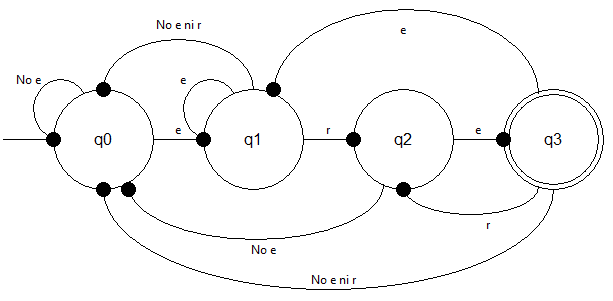
\includegraphics[width=14cm, height=7cm]{img/ere.png}
		\caption{Diagrama de transiciones del autómata 'ere'.}
		\label{fig:diagrama1}
		\end{center}
	\end{figure}
	\subsection{Código}
	El código fue realizado en Python 3.5.
	\\Archivo: main\_ere.py
	\begin{lstlisting}[language=Python]
	#main_ere.py
	# -*- coding: utf-8 -*-
	from __future__ import print_function
	from automata_ere import verificar_palabras
	from diagrama_ere import Diagrama
	
	separador = '*'*50
	
	def iniciar():
		continuar = True
		while continuar:
			opcion = imprimir_menu()
			if opcion == 1:
				entrada_consola()
			elif opcion == 2:
				entrada_archivo()
			elif opcion == 3:
				ver_diagrama()
			else:
				break
			print('*' * 100)
			opcion = input("Reintentar s/n: ")
			if opcion.lower() != 's':
				continuar = False
		
		print('Saliendo del programa...')
	
	def imprimir_menu():
		print("""Es importante mencionar que en este programa cualquier simbolo que no sea una letra en el alfabeto ingles separa una palabra de otra""")
		print('\n\n%sMenu%s' % (separador, separador))
		print("""
		1.- Entrada en consola
		2.- Ingresar nombre del archivo
		3.- Ver diagrama de estados
		4.- Salir
		""")
		try:
			opcion = int(input("Selecciona una opcion valida: "))
			return opcion
		except Exception as e:
			print('Error ', e)
			return 0
	
	def entrada_consola():
		texto = input("Escribe el texto: ")
		texto += ' '
		palabras_ere = []
		verificar_palabras(texto, palabras_ere)
		print('\n', palabras_ere)
	
	def entrada_archivo():
		archivo = input("Ingresa el nombre del archivo: ")
		try:
			archivo_abierto = open(archivo, 'r')
		except Exception as e:
			print('Error al abrir archivo: ', e)
			return 0
		
		linea_palabras = []
		num_linea = 1
		palabras_ere = []
		posiciones = []
		for linea in archivo_abierto:
			verificar_palabras(linea, palabras_ere, posiciones)
			linea_palabras.append({'Linea': num_linea, 'Palabras': palabras_ere, 'Posiciones': posiciones})
			num_linea += 1
			palabras_ere = []
			posiciones = []
		
		imprimir_archivo(linea_palabras)
		archivo_abierto.close()
	
	def imprimir_archivo(linea_palabras):
		print('\n\n')
		for elemento in linea_palabras:
			if len(elemento['Palabras']) > 0:
				print('Numero de linea: ', elemento['Linea'])
				i = 0
				for palabra in elemento['Palabras']:
					print('\tPalabra: %s No. Palabra: %s' % (palabra, elemento['Posiciones'][i]))
					i += 1
	
	def ver_diagrama():
		print('Mostrando diagrama del automata. Cierre la ventana para continuar')
		try:
			diagrama_ere = Diagrama()
			diagrama_ere.master.title('Diagrama del automata ere')
			diagrama_ere.mainloop()
		except Exception as e:
			print("Error", e)
	
	iniciar()
	\end{lstlisting}
	Archivo: automata\_ere.py
	\begin{lstlisting}[language=Python]
	#automata_ere.py
	# -*- coding: utf-8 -*-
	from __future__ import print_function
	
	def verificar_palabras(texto, palabras_ere, posiciones = []):
		palabra_aux = ''
		estado = 0
		num_palabra = 1
		for simbolo in texto:
			simbolo_aux = simbolo.lower()
			if simbolo ==  '\n':
				simbolo = '\\n'
			print('-> delta(q%s,%s)' % (estado, simbolo), end="\t")
			
			estado = automata(estado, simbolo_aux)
			
			if (ord(simbolo_aux) < 123 and ord(simbolo_aux) > 96):
				palabra_aux += simbolo
				if estado == 4:
					estado = 0
			else:
				if estado == 4:
					palabras_ere.append(palabra_aux)
					posiciones.append(num_palabra)
					estado = 0
				palabra_aux = ''
				if simbolo == ' ':
					num_palabra += 1
	
	def automata(estado, simbolo):
		if estado == 0:
			estado = estado_cero(simbolo)
		elif estado == 1:
			estado = estado_uno(simbolo)
		elif estado == 2:
			estado = estado_dos(simbolo)
		elif estado == 3:
			estado = estado_tres(simbolo)
		else:
			print('Simbolo extrano: ', simbolo)
		
		return estado
	
	def estado_cero(simbolo):
		if simbolo == 'e':
			return 1
		else:
			return 0
	
	def estado_uno(simbolo):
		if simbolo == 'r':
			return 2
		elif simbolo == 'e':
			return 1
		else:
			return 0
	
	def estado_dos(simbolo):
		if simbolo == 'e':
			return 3
		else:
			return 0
	
	def estado_tres(simbolo):
		if simbolo == 'r':
			return 2
		elif simbolo == 'e':
			return 1
		else:
			return 4
	\end{lstlisting}
	Archivo: diagrama\_ere.py
	\begin{lstlisting}[language=Python]
	#diagrama_ere.py
	# -*- coding: utf-8 -*-
	from __future__ import print_function
	import tkinter as tk
	
	class Diagrama(tk.Frame):
		def __init__(self, master=None):
			super().__init__(master, background='white')
			self.pack(fill=tk.BOTH, expand=tk.YES)
			self.dibujarDiagrama()
			self.centrarVentana()
	
		def dibujarDiagrama(self):
			canvas = tk.Canvas(self, bg='white')
			datos = {}
			datos['coordenadas'] = [100, 100, 200, 200]
			datos['canvas'] = canvas
			self.circulos_flechas(datos)
			
			self.crear_arco(canvas, [150, 50, 300, 150])
			canvas.create_text(150+75, 50-15, text='No e ni r')
			self.crear_arco(canvas, [320, 20, 585, 190])
			canvas.create_text(320+130, 50-10, text='e')
			# reflexiva
			extra = {'start': 30, 'extend': 235}
			self.crear_arco(canvas, [80, 90, 135, 150], extra)
			canvas.create_text(80-5, 90, text='No e')
			self.crear_arco(canvas, [230, 90, 285, 150], extra)
			canvas.create_text(230, 90, text='e')
			
			#de cabeza
			extra = {'start': 0, 'extend': -180}
			self.crear_arco(canvas, [150, 100, 600, 300], extra)
			canvas.create_text(600-220, 300-10, text='No e ni r')
			self.crear_arco(canvas, [175, 140, 430, 250], extra)
			canvas.create_text(430-120, 300-40, text='No e')
			self.crear_arco(canvas, [450, 170, 585, 225], extra)
			canvas.create_text(585-50, 225+10, text='r')
			
			canvas.pack(fill=tk.BOTH, expand=1)
		
		def circulos_flechas(self, arg):
			coordenadas = arg['coordenadas']
			canvas = arg['canvas']
			for x in range(4):
				self.escribirTexto(canvas, x, coordenadas)
				self.dibujarCirculo(canvas, coordenadas)
				self.dibujarFlecha(canvas, [coordenadas[0]-50, 150, coordenadas[2]-100, 150])
				coordenadas[0] += 150
				coordenadas[2] += 150
			
			self.dibujarCirculo(canvas, [coordenadas[0]-150+5, 105, coordenadas[2]-155, 195]) # circulo interior
		
		def escribirTexto(self, canvas, x, coordenadas):
			text = ''
			text_flecha =''
			if x == 0:
				text = 'q%s' % x
				text_flecha = ''
			elif x == 1:
				text = 'q%s' % x
				text_flecha = 'e'
			elif x == 2:
				text = 'q%s' % x
				text_flecha = 'r'
			elif x == 3:
				text = 'q%s' % x
				text_flecha = 'e'
			else:
				print('otro')
		
			canvas.create_text(coordenadas[0]+50, coordenadas[1]+50, font=('15'), text=text)
			canvas.create_text(coordenadas[0]-25, coordenadas[1]+40, text=text_flecha)
		
		def dibujarCirculo(self, canvas, coordenadas):
			circulo = canvas.create_oval(coordenadas)
		
		def dibujarFlecha(self, canvas, coordenadas):
			linea = canvas.create_line(coordenadas)
			canvas.create_oval(coordenadas[2]-7, coordenadas[1]-7, coordenadas[2]+7,coordenadas[1]+7, fill = 'black')
		
		def crear_arco(self, canvas, coordenadas, extra=None):
			if extra != None:
				arco = canvas.create_arc(coordenadas, start=extra['start'], extent=extra['extend'], style='arc')
				if extra['extend'] == -180:
					canvas.create_oval(coordenadas[0]-7, 100+100-7, coordenadas[0]+7, 100+100+7, fill = 'black')
			else:
				arco = canvas.create_arc(coordenadas, start=0, extent=180, style='arc')
				canvas.create_oval(coordenadas[0]-7, 100-7, coordenadas[0]+7, 100+7, fill = 'black')
		
		def centrarVentana(self):
			ancho, altura = 700, 350
			ancho_pantalla = self.winfo_screenwidth()
			altura_pantalla = self.winfo_screenheight()
			posicion_x = (ancho_pantalla - ancho)/2
			posicion_y = (altura_pantalla - altura)/2
			self.master.geometry('%dx%d+%d+%d' % (ancho, altura, posicion_x, posicion_y))
	
	\end{lstlisting}
	\subsection{Pruebas}
	Pruebas de las opciones del menú.
	\\
	{\large Modo de consola.}
	\begin{figure}[H]
		\begin{center}
			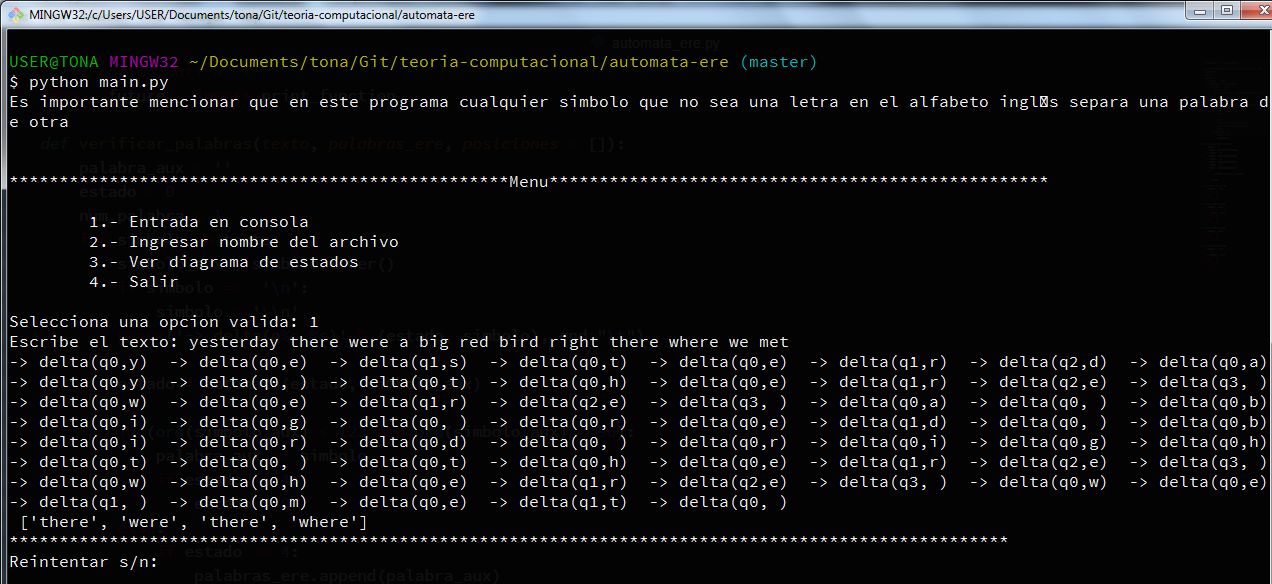
\includegraphics[width=\linewidth, height=6cm]{img/ere-manual.png}
			\caption{Historia del autómata y las palabras con terminación 'ere'.}
			\label{fig:ere1}
		\end{center}
	\end{figure}
	{\large Modo archivo.}
	\begin{figure}[H]
		\begin{center}
			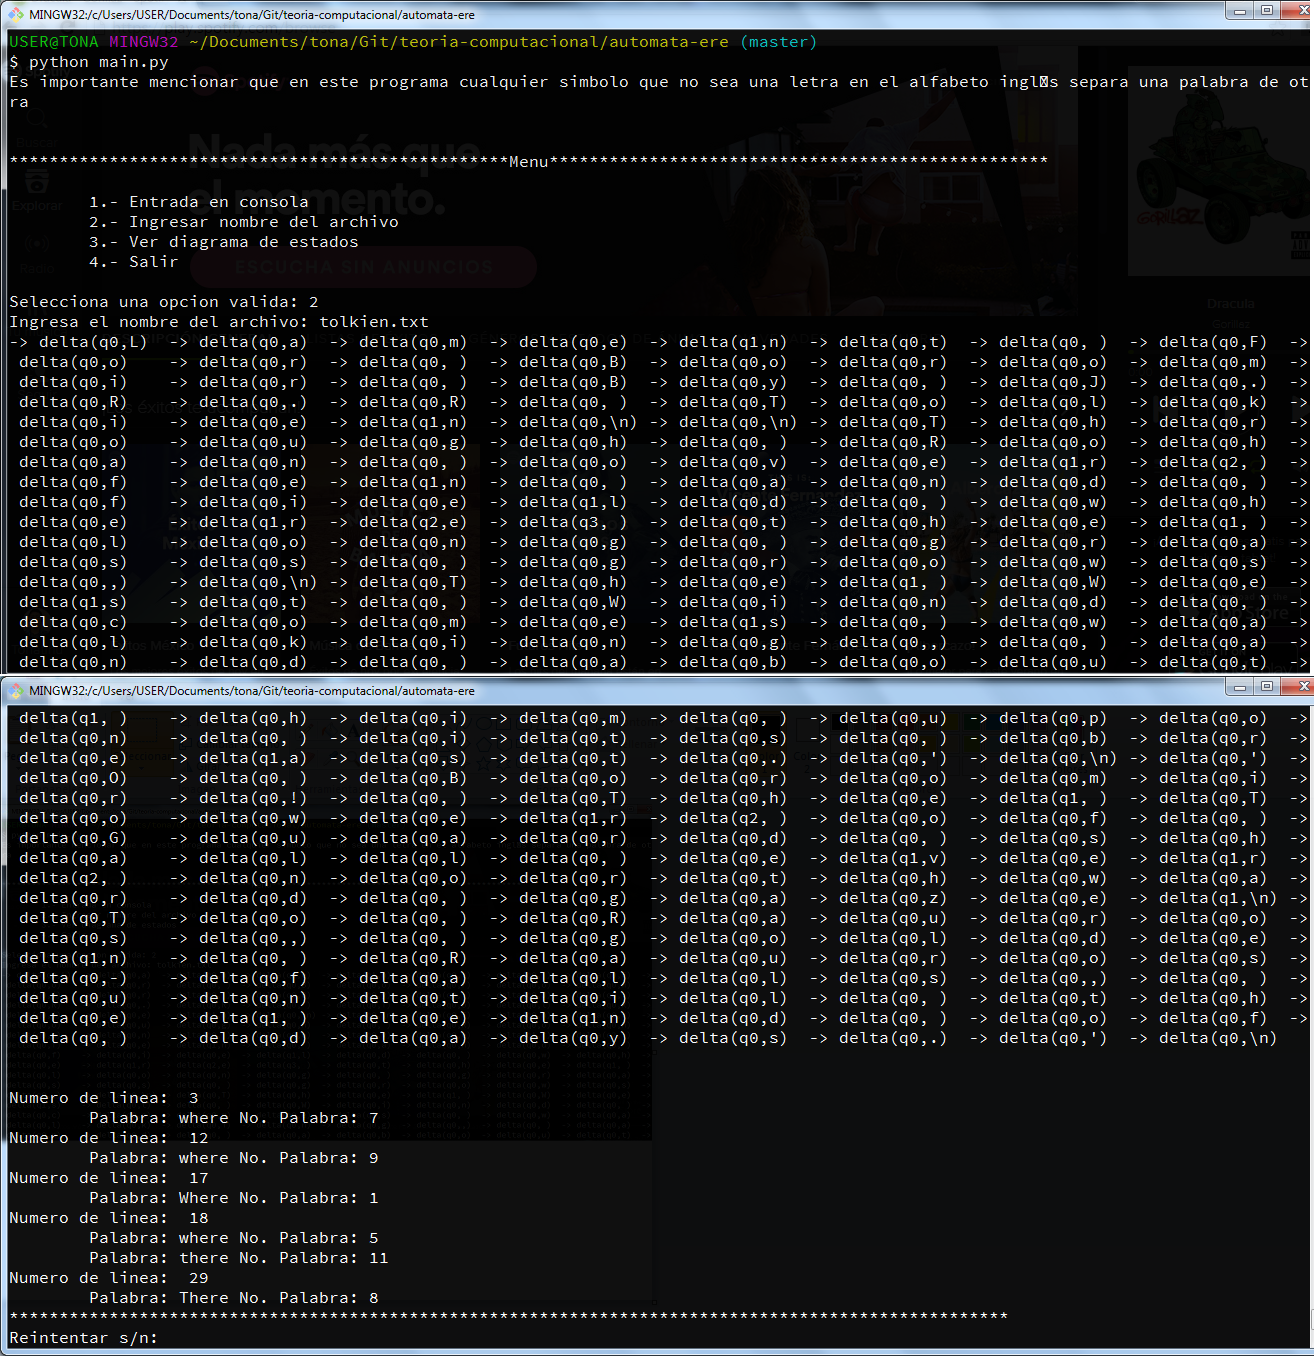
\includegraphics[width=\linewidth, height=20cm]{img/ere-automatico.png}
			\caption{Parte de la historia del autómata y las palabras con terminación 'ere'.}
			\label{fig:ere2}
		\end{center}
	\end{figure}
	{\large Diagrama.}
	\begin{figure}[H]
		\begin{center}
			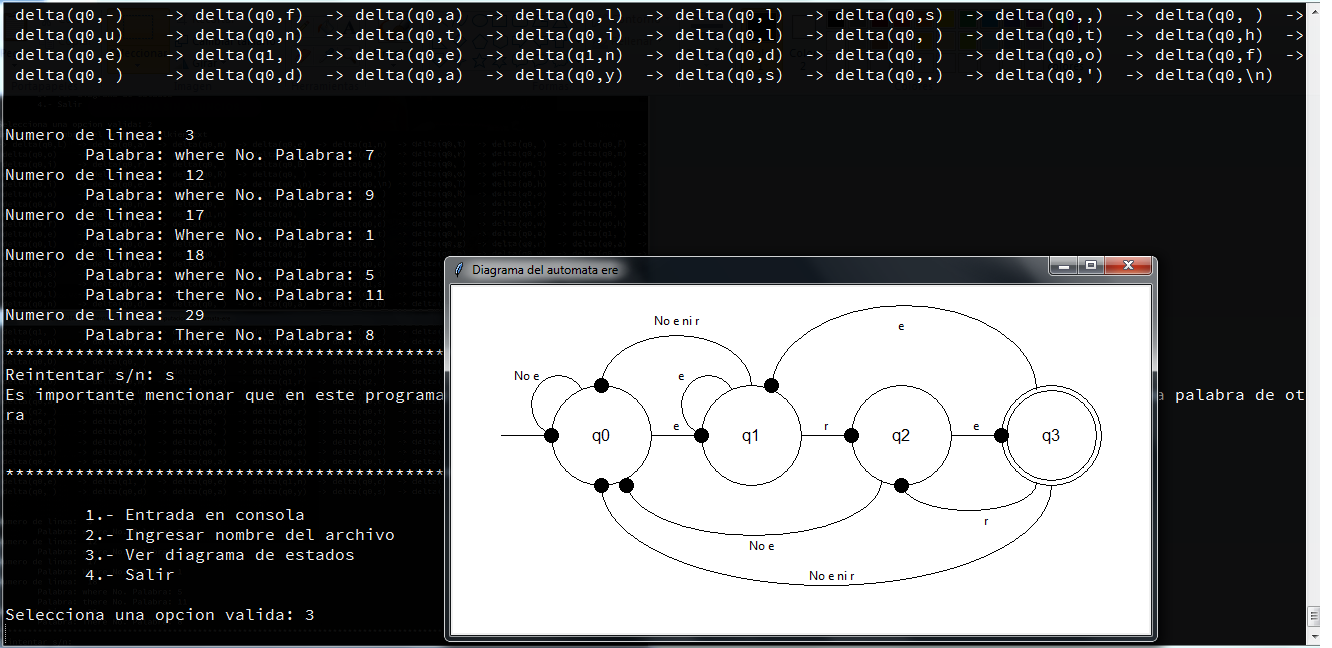
\includegraphics[width=\linewidth, height=9cm]{img/diagrama-ere.png}
			\caption{Diagrama de transiciones del autómata 'ere'.}
			\label{fig:ere3}
		\end{center}
	\end{figure}